\documentclass[12pt]{article}
\usepackage[utf8]{inputenc}
\usepackage[margin=1in]{geometry}
\usepackage{amssymb}
\usepackage{amsmath}
\usepackage{mathtools}
\usepackage{amsthm}
\usepackage{setspace}
\usepackage{cancel}
\usepackage{bbm}
\usepackage{pgfplots}
\usetikzlibrary{arrows, calc, patterns, shapes}
  \pgfplotsset{compat=1.15}
\renewcommand{\baselinestretch}{1.25}
\newcommand\sbullet[1][.5]{\mathbin{\vcenter{\hbox{\scalebox{#1}{$\bullet$}}}}}
\newcommand{\indep}{\perp \hspace{-.5 em} \perp}
\def\E{\mathbb{E}}
\def\e{\mathcal{E}}
\def\d{\mathcal{D}}
\def\I{I_n}
\def\l{\ell}
\def\sumn{\sum^n_{i=1}}
\def\i{\mathcal{J}}
\def\x{\mathbf{X}}
\def\inv{^{-1}}
\newcommand{\til}[1]{\underset{\sim}{#1}}
\newcommand\expp[1]{\exp\bigg\{#1\bigg\}}
\newcommand\der[2]{\frac{\partial #1}{\partial #2}}
\newcommand{\ds}{\displaystyle}

\theoremstyle{definition}
\newtheorem{theorem}{Theorem}

\theoremstyle{definition}
\newtheorem{definition}{Definition}

\newtheorem{example}{Example}[section]

\let\inf\infty
\title{Math 410}
\author{--- }
\date{September 2019}

\begin{document}

\maketitle
\tableofcontents{}
\pagebreak

\section{Necessary Background }

\subsection{Brief Introduction to Bayesian Networks}
The goal of Bayesian Networks is to represent a joint distribution over a set of random variables using a directed acyclic graph. Let $\mathcal{D}=(V,E)$ be such a graph. The set of nodes $V$ will represent random variables and the set of edges $E$ will correspond to the direct influence between two nodes. Intuitively, edge orientation can be interpreted at a causal relation between two rvs.

\noindent
When working with Bayesian Networks, nodes (rvs) are independent from other nodes given their immediate parents. This is referred to as the \textbf{Markov property}.
\begin{center}
\tikzset{every picture/.style={line width=0.75pt}}
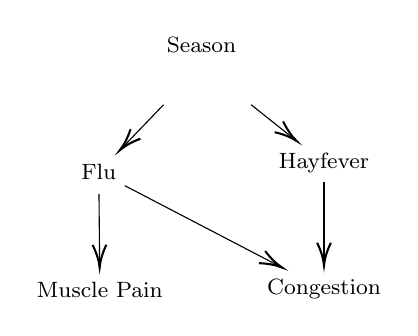
\begin{tikzpicture}[x=0.75pt,y=0.75pt,yscale=-1,xscale=1]
\draw (225,56) node  [align=left] {{\footnotesize Season}\\};
\draw (175.5,107.5) node  [align=left] {{\footnotesize Flu}};
\draw (284,103) node  [align=left] {{\footnotesize Hayfever}};
\draw (284,164) node  [align=left] {{\footnotesize Congestion}};
\draw (176,164) node  [align=left] {{\footnotesize Muscle Pain}};
\draw    (206.74,75) -- (186.98,95.56) ;
\draw [shift={(185.59,97)}, rotate = 313.87] [color={rgb, 255:red, 0; green, 0; blue, 0 }  ][line width=0.75]    (10.93,-3.29) .. controls (6.95,-1.4) and (3.31,-0.3) .. (0,0) .. controls (3.31,0.3) and (6.95,1.4) .. (10.93,3.29)   ;
\draw    (248.85,75) -- (269.25,91.25) ;
\draw [shift={(270.82,92.5)}, rotate = 218.54] [color={rgb, 255:red, 0; green, 0; blue, 0 }  ][line width=0.75]    (10.93,-3.29) .. controls (6.95,-1.4) and (3.31,-0.3) .. (0,0) .. controls (3.31,0.3) and (6.95,1.4) .. (10.93,3.29)   ;
\draw    (188,114.01) -- (262.06,152.58) ;
\draw [shift={(263.84,153.5)}, rotate = 207.51] [color={rgb, 255:red, 0; green, 0; blue, 0 }  ][line width=0.75]    (10.93,-3.29) .. controls (6.95,-1.4) and (3.31,-0.3) .. (0,0) .. controls (3.31,0.3) and (6.95,1.4) .. (10.93,3.29)   ;
\draw    (175.59,118) -- (175.89,151.5) ;
\draw [shift={(175.91,153.5)}, rotate = 269.49] [color={rgb, 255:red, 0; green, 0; blue, 0 }  ][line width=0.75]    (10.93,-3.29) .. controls (6.95,-1.4) and (3.31,-0.3) .. (0,0) .. controls (3.31,0.3) and (6.95,1.4) .. (10.93,3.29)   ;
\draw    (284,112.5) -- (284,150.5) ;
\draw [shift={(284,152.5)}, rotate = 270] [color={rgb, 255:red, 0; green, 0; blue, 0 }  ][line width=0.75]    (10.93,-3.29) .. controls (6.95,-1.4) and (3.31,-0.3) .. (0,0) .. controls (3.31,0.3) and (6.95,1.4) .. (10.93,3.29)   ;
\end{tikzpicture}
\end{center}
By the Markov property,  BN above represents the following joint probability:
$$P(s,f,h,m,c)=P(s)P(f|s)P(h|s)P(m|f)P(c|f,h)$$

\subsection{Monoid}
A set $S$ with a binary operator $\bullet : S \times S \rightarrow S $ is a \textbf{monoid} if it satisfies the following properties:
\begin{itemize}
    \item \textbf{Associativity:} $\forall a,b,c \in S, (a\bullet b)\bullet c = a \bullet (b\bullet c)$ 
    \item \textbf{Identity Element} $\exists e \in S\ \  s.t.\  \forall a\in S, e \bullet a =a \bullet e = a$
\end{itemize}

\subsection{Semiring}
A \textbf{semiring} $(R,\bigvee,\cdot)$ is defined by a set $R$ and two of its operators with the following properties:
\begin{itemize}
    \item $(R,\bigvee) $ is a commutative monoid with identity 0
    \item $(R,\cdot)$ is a monoid with identity 1
\end{itemize}
In the contex of max-linear models, we will be using $\bigvee$ as the max operator, and $\cdot$ as the matrix product.

\section{Introduction to Max-Linear Models}
\subsection{Recursive Structural Equation Model}
Given a DAG $\mathcal{D}=(V,E)$ with nodes $V=\{1,\hdots, d\}$ and edges $E=\{(k,i):i \in V \ \text{and } K \in pa(i)\}$, we define a \textbf{recursive structural equation model} to be any function $$X_i=f_i(X_{pa(i)},Z_i)$$

\begin{itemize}
    \item with $ \ds pa(i)$ denoting the direct parents of node $i$ in $\mathcal{D}$
    \item $f_i$ as a real valued measurable function
    \item $\ds \{ Z_1, \hdots , Z_d\}$ as independent noise variables\footnote{The distribution $\mathbf{X}$ is uniquely determined by these noise variables}
\end{itemize}
By analyzing the set of equations, $\mathbf{X}= (X_1, \hdots, X_d)$, we can see why this model has its name. $\x$ is recursively generated and, through parentage, the generation of each successive $X_i$ is driven by the structure of the graph.

\noindent Let $nd(i)$ denote the set of non-descendants of $i$ then, by construction, 
$$X_i \indep X_{nd(i)\setminus pa(i)}|X_{pa(i)} \ \ \ i=1,\hdots, d$$
 which means that the distribution on $\mathbf{X}$ is Markov with respect to $\mathcal{D}$.
 
\subsection{Recursive Max-Linear Model}
 This model is motivated by its applications to risk analysis and the tendency of risk to propagate through a network. The \textbf{recursive max-linear model} $\x=(X_1,\hdots, X_d)$ on a DAG $\mathcal{D}$ is defined as:
$$X_i:= \bigvee_{k\in pa(i)}c_{ki}X_k \vee c_{ii}Z_i\ \ \  i=1,\hdots,d$$
\begin{itemize}
    \item $\ds \{c_{ki} \forall i \in V \text{and } k \in pa(i)\cup\{i\}\}$ as positive weights 
    \item $\{Z_1, \hdots Z_d\}$ as independent, non negative rvs with positive and infinite support.
\end{itemize}
The weights represent relative quantities that a risk originates with a certain proportion in different ancestors.

\subsubsection{Max-Linear Coefficient Matrix}
\noindent This model can be re-written in the form $$X_i:= \bigvee_{j=1}^db_{ji}Z_j\ \ \  i=1,\hdots,d$$
$B=(b_{ij})_{d\times d}$ is a matrix with non-negative entries called the \textbf{max linear coefficient matrix} of $\x$ and its entries are dubbed \textbf{max-linear coefficients}. The construction of the matrix $B$ is fairly intuitive. First, for any two nodes $(j,i)$ we assign a weight to every path $p= [j=k_0\rightarrow k_1\rightarrow \hdots \rightarrow k_n=i]$. This weight is equal to the edge product allong the path $p$ multiplied by the noise variable (denoted $Z_j$) associated with the starting node $j$. Below is an equation that might assist in visualizing the edge product $d_{ji}(p)$:
$$d_{ji}(p):=c_{k_0,k_0}\cdot c_{k_0,k_1}\cdot\hdots\cdot c_{k_{n-2},k_{n-1}}\cdot c_{k_{n-1},k_n}=c_{k_0,k_0}\prod_{l=0}^{n-1}c_{k_l,k_{l+1}}$$
Let $an(i)$ denote the ancestors of a node, $An(i)=an(i)\cup\{i\}$, and $P_{ji}$ denote all possible paths from node $j$ to node $i$. Then, the ML coefficients for any $i\in V$ are given by:
\begin{align*}
    b_{ii}&= c_{ii}\\
    b_{ji}&=\bigvee_{p\in P_{ji}}d_{ji} \text{ for }j\in an(i)\\
    b_{ji}&=0 \text{ for } j \in V \setminus An(i)
\end{align*}
\begin{itemize}
 \item The coefficient between a node $i$ and itself is simply the weight $c_{ii}$
    \item The coefficient between any two nodes $(j,i)$ is given by the path with the largest weight
    \item The coefficient between any two nodes with no path between them is $0$
\end{itemize}
From our construction, our new model for $X_i$ comes with a slightly new explanation. In \textit{"pseudo stats"}, the model is given by :
$$X_i=\max_{\text{for all nodes }j\in V}\bigg( \max(\text{path weight between nodes }i \text{ and }j ) * \text{noise associated to }j\bigg) $$
\pagebreak

\subsubsection{Example of Max-Linear Model}
Let $\d=(V,E)=(\{1,2,3,4\}, \{(1,2),(1,3), (2,4),(3,4)\})$, and $C=\{c_{ik}: i\in V, k\in pa(i)\}$. Now, let us build the recursive ML model $\x= (X_1,X_2,X_3,X_4)$\\
\begin{minipage}{0.5 \linewidth}
$ 
\begin{aligned}[t] 
X_1&= c_{11}Z_1\\
X_2&= c_{12}X_1\vee c_{22}Z_2 =c_{12}c_{11}Z_1 \vee c_{22}Z_2\\
X_3&= c_{13}X_1\vee c_{33}Z_3 =c_{13}c_{11}Z_1 \vee c_{33}Z_3\\
X_4&= c_{24}X_2\vee c_{34}X_3\vee c_{44}Z_4\\
&=c_{24}(c_{12}c_{11}Z_1 \vee c_{22}Z_2)\vee c_{34}(c_{13}c_{11}Z_1 \vee c_{33}Z_3)\vee c_{44}Z_4\\
&=(c_{24}c_{12}c_{11}\vee c_{34}c_{13}c_{11})Z_1 \vee (c_{24}c_{22})Z_2\vee (c_{34}c_{33})Z_3 \vee c_{44}Z_4\\
\end{aligned}
$
\end{minipage}
\begin{minipage}{0.2 \linewidth}
~
\end{minipage}
\begin{minipage}{0.45 \linewidth}
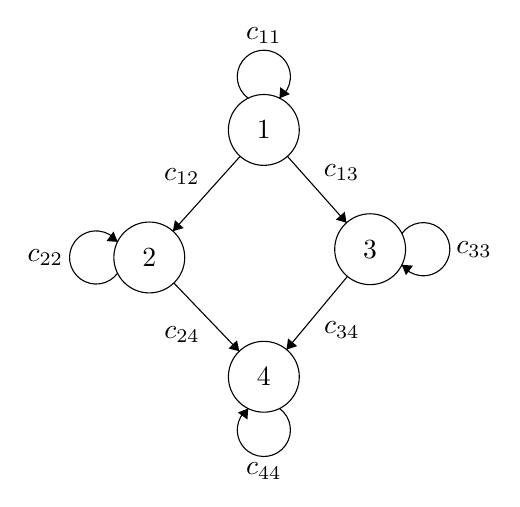
\begin{tikzpicture}[scale=0.15,
baseline={(current bounding box.center)}]
\tikzstyle{every node}+=[inner sep=0pt]
\draw [black] (36.2,-11.6) circle (3);
\draw (36.2,-11.6) node {$1$};
\draw [black] (26.5,-22.4) circle (3);
\draw (26.5,-22.4) node {$2$};
\draw [black] (45.2,-21.7) circle (3);
\draw (45.2,-21.7) node {$3$};
\draw [black] (36.2,-32.5) circle (3);
\draw (36.2,-32.5) node {$4$};
\draw [black] (34.2,-13.83) -- (28.5,-20.17);
\fill [black] (28.5,-20.17) -- (29.41,-19.91) -- (28.67,-19.24);
\draw (30.81,-15.54) node [left] {$c_{12}$};
\draw [black] (34.877,-8.92) arc (234:-54:2.25);
\draw (36.2,-4.35) node [above] {$c_{11}$};
\fill [black] (37.52,-8.92) -- (38.4,-8.57) -- (37.59,-7.98);
\draw [black] (38.2,-13.84) -- (43.2,-19.46);
\fill [black] (43.2,-19.46) -- (43.05,-18.53) -- (42.3,-19.2);
\draw (41.24,-15.19) node [right] {$c_{13}$};
\draw [black] (23.82,-23.723) arc (324:36:2.25);
\draw (19.25,-22.4) node [left] {$c_{22}$};
\fill [black] (23.82,-21.08) -- (23.47,-20.2) -- (22.88,-21.01);
\draw [black] (28.58,-24.56) -- (34.12,-30.34);
\fill [black] (34.12,-30.34) -- (33.93,-29.41) -- (33.21,-30.11);
\draw (30.82,-28.92) node [left] {$c_{24}$};
\draw [black] (43.28,-24) -- (38.12,-30.2);
\fill [black] (38.12,-30.2) -- (39.02,-29.9) -- (38.25,-29.26);
\draw (41.25,-28.54) node [right] {$c_{34}$};
\draw [black] (47.88,-20.377) arc (144:-144:2.25);
\draw (52.45,-21.7) node [right] {$c_{33}$};
\fill [black] (47.88,-23.02) -- (48.23,-23.9) -- (48.82,-23.09);
\draw [black] (37.523,-35.18) arc (54:-234:2.25);
\draw (36.2,-39.75) node [below] {$c_{44}$};
\fill [black] (34.88,-35.18) -- (34,-35.53) -- (34.81,-36.12);
\end{tikzpicture}
\end{minipage}
\break
\noindent 
Our vector $\x$ is a ML model with ML coefficient matrix 
\[ B=\begin{bmatrix}
&c_{11} &c_{12}c_{11} & c_{13}c_{11}& c_{24}c_{12}c_{11}\vee c_{34}c_{13}c_{11}\\
&0 & c_{22} & 0& c_{22}c_{24}\\
&0&0 &c_{33} & c_{33}c_{34} \\
&0& 0 & 0 & c_{44}\\
\end{bmatrix}
\]
To visualize the generation of this matrix given a graph $\d$ and weights $C$, please consult r code.

\pagebreak

\section{Model Distribution}
Now that we have the model, our goal is to find the underlying distribution of each of the $X_i$. To do this, we need a stronger tool than the ones at our disposal.

\subsection{Copulas}
A \textbf{Copula} is a cumulative distribution function with univariate, uniform margins\footnote{ref Copula and copula models}. This term is derived from Latin and refers to a link. In this context, copulas help to determine the dependence between random variables.

\noindent \begin{theorem}[Sklar's Theorem] Given random variables $X_1,\hdots,X_d$ with cumulative distribution functions $F_1,\hdots,F_d$, there always exists a copula $C$ such that 
$$P(X_1\leq x_1, \hdots, X_d\leq x_d)=C( F_1(x_1),\hdots ,F_d(x_d))\hspace{1cm}\forall x_1\hdots,x_d\in\mathbb{R}$$
This means that the joint cumulative distribution of random variables $\ds \{X_i\}_{i=1}^d $ can be represented by a function of the marginal probability distributions.
\end{theorem}
\begin{theorem}[Extension to Sklar's Theorem]
If the cumulative distribution functions are continuous, then the copula $C$ is unique and can be retrieved by the joint cdf of the original random variable vector $(X_1,\hdots,X_d)$ after the \textbf{integral transform} has been applied to each of the components: $(F_1(X_1),\hdots,F_d(X_d))$.
\begin{proof}
In this paper, we show this result holds for the set of continuous and strictly increasing functions $\ds \{F_i\}_{i=1}^d$. The result also holds for monotonic increasing functions but is slightly harder to show.
From the restriction on the functions, we know that $\forall x,y \in \mathbb{R} ,\forall i\ s.t.\ 1\leq i\leq d$ we have $x\leq y\implies F_i(x)\leq F_i(y)$. We can now use this to prove our result. 
\begin{align*}
    C( F_1(x_1),\hdots ,F_d(x_d))&=P(X_1\leq x_1,\hdots, X_d\leq x_d)\\
    &=P(F_1(X_1)\leq F_1(x_1),\hdots,F_d(X_d)\leq F_d(x_d))\\
    &=P(F_1(X_1)\leq u_1,\hdots,F_d(X_d)\leq u_d)\\
    &=P(X_1\leq F_1^{-1}(u_1),\hdots,X_d\leq F_d^{-1}(u_d))\\
    &=C(F_1(F_1^{-1}(u_1)),\hdots,F_d(F_d^{-1}(u_d)))\\
    &=C(u_1,\hdots,u_d)
\end{align*}
From this we note that the copula can be set to the joint cdf of the random vector obtained by element wise integral transform.
\end{proof}

\end{theorem}


\subsection{Copulas and ML-Models}
Let us assume that we have data that consists of  $n$ observations from $d$ sources denoted $X_1,\hdots, X_d$. If we want to use a ML model to learn more about the underlying structure and relationship between these sources, we make use of copulas. To calculate the copulas, we must calculate the following:
\begin{enumerate}
    \item The marginal cdfs $\ds\{F_1, \hdots, F_d\}$ \item The joint cdf $H(x_1,\hdots,x_d)=P(X_1\leq x_1, \hdots, X_d\leq x_d)$
    \item The copula $C(u_1,\hdots,c_d)=H(F\inv_1(u_1),\hdots,F\inv_d(u_d))$
\end{enumerate}

\subsubsection{Marginal cdfs (theory)}
Assume the random variables $X_1,\hdots, X_d$ follow a ML model with i.i.d shock random variables $Z_1,\hdots, Z_d$ and ML coefficient matrix 
\[ B=\begin{bmatrix}
&b_{11} &b_{12}&\hdots& b_{1d-1}& b_{1d}\\
&b_{21} &b_{22}&\hdots& b_{2d-1}& b_{2d}\\
&\vdots&\vdots&\ddots & \vdots& \vdots \\
&\vdots&\vdots&\hdots & \ddots& \vdots \\
&b_{d1}& b_{d2} & \hdots &b_{d-1}& b_{d}\\
\end{bmatrix}
\]
Where $b_{ij}$ is the maximum weight associated with any path from $i$ to $j$. We can calculate the marginal cdf for each of the $X_k$:
\begin{align*}
    F_{X_k}(x_k)&=P(X_k\leq x_k)\\
    &=P(\bigvee_{j=1}^db_{jk}Z_j\leq x_k)\\
    &=\prod_{j=1}^dP(Z_j\leq \frac{x_k}{b_{jk}})\\
    &=\prod_{j=1}^dF_{Z_j}( \frac{x_k}{b_{jk}})
\end{align*}
Now, if we assume that $Z_i\overset{iid}{\thicksim}$ Fréchet $(\alpha)$ we get the following result
\begin{align*}
    F_{k}(x_k)&=\prod_{j=1}^d\exp\bigg\{{-\big(\frac{x_k}{b_{jk}}}\big)^{-\alpha}\bigg\}\\
    &=\exp\bigg\{{-\sum_{j=1}^d\big(\frac{x_k}{b_{jk}}}\big)^{-\alpha}\bigg\}\\
    &=\exp\bigg\{{-x_k^{-\alpha}\sum_{j=1}^d{b_{jk}}^{\alpha}}\bigg\}\\
    \implies F_{k}\inv(u)&=\bigg(\frac{\sum_{j=1}^d{b_{jk}^\alpha}}{-\log(u)} \bigg)^{{1}/{\alpha}}
\end{align*}
It is important to note that if $j\notin An(k)$ then $b_{jk}=0$. This means that the sum $\ds \sum_{j=1}^d{b_{jk}}$ is equivalent to $\ds \sum_{j\in An(k)}{b_{jk}}$.
\subsubsection{Marginal cdfs (from data)}
From the data, we have $$\{(X_{11},\hdots,X_{1d}), \hdots, (X_{n1}, \hdots X_{nd})\}$$To build a copula, we need the points 
$$\{(F_1(X_{11}),\hdots,F_d(X_{1d})), \hdots, (F_1(X_{n1}), \hdots F_d(X_{nd}))\}$$
To represent a sample from $C$, because we do not have the analytic values for $\{F_1,\hdots,F_d\}$, we estimate them using the following formula:
$$\widehat{F}_i(x)=\frac{1}{n}\sum_{j=1}^n\mathbbm{1}(X_{ij}\leq x)$$
This is an application of the \textbf{rank plot} method. Essentially, for each random variable $X_{i}$, we rank all observations from smallest to greatest. Then, the rank (position in observation vector) of each observation helps us build our cdf $F_i$. The marginal cdf of each random variable evaluated at $x$ is calculated by dividing the number of observations greater than $x$ by the total number of observations. In practice, we use 
$$\widehat{F}_i(x)=\frac{1}{n+1}\sum_{j=1}^n\mathbbm{1}(X_{ij}\leq x)$$
because it leads to nicer results.
\subsubsection{Joint cdf}
In general, the joint cdf $H$ of random variables following a max-linear model can be calculated in the following way:
\begin{align*}
    H(x_1,\hdots, x_d)&=P(X_1\leq x_1,\hdots,X_d\leq x_d)\\
    &=P(\bigvee_{j=1}^db_{j1}Z_j\leq x_1, \hdots, \bigvee_{j=1}^db_{jd}Z_j\leq x_d)\\
    &=P(Z_1\leq{\bigwedge_{k=1}^d\frac{x_k}{b_{1k}}},\hdots, Z_d\leq\bigwedge_{k=1}^d\frac{x_k}{b_{dk}})\\
    &=\prod_{i=1}^dF_i(\bigwedge_{k=1}^d\frac{x_k}{b_{ik}})
\end{align*}
When we deal with Frechét shock, this simplifies.
\begin{align*}
    F_i(\bigwedge_{k=1}^d\frac{x_k}{b_{ik}})&=\exp\bigg\{-\bigg(\bigwedge_{k=1}^d\frac{x_k}{b_{ik}}\bigg)^{-\alpha}\bigg\}\\
    &=\exp\bigg\{-\bigvee_{k=1}^d \bigg( \frac{b_{ik}}{x_k} \bigg)^\alpha\bigg\}\\
    \implies H(x_1,\hdots, x_d)&=\prod_{i=1}^d\exp\bigg\{-\bigvee_{k=1}^d \bigg( \frac{b_{ik}}{x_k} \bigg)^\alpha\bigg\}\\
    &=\exp\bigg\{ -\sum_{i=1}^d \bigvee_{k=1}^d \bigg( \frac{b_{ik}}{x_k} \bigg)^\alpha \bigg\}\\
    &=\exp\bigg\{ -\sum_{i=1}^d \bigvee_{k=1}^d \bigg( \frac{b_{ik}}{x_k} \bigg)^\alpha \bigg\}
\end{align*}
Again we note that the index of the max operator can be changed to be in terms of ancestors. This is because for any two random variables $i,k$, if $i \notin An(k)$, then $b_{ik}=0$. So we can write 
$$H(x_1,\hdots,x_d)=\exp\bigg\{ -\sum_{k=1}^d  \bigvee_{i\in An(k)}\bigg( \frac{b_{ik}}{x_k} \bigg)^\alpha \bigg\}$$

\subsubsection{Building the Copula}
Now, we can put it all together to find the copula.
\begin{align*}
    C(u_1,\hdots, u_d)&=H(F_1\inv(u_1),\hdots, F_d\inv(u_d))\\
\end{align*}
When dealing with Frechét shock, the calculation becomes:
\begin{align*}
a_k&=\sum_{j=1}^d{b_{jk}^\alpha}\\
F_{k}\inv(u)&=\bigg(\frac{\sum_{j=1}^d{b_{jk}^\alpha}}{-\log(u)} \bigg)^{{1}/{\alpha}}=\bigg(\frac{a_k}{- \log(u)}\bigg)^{1/\alpha}\\
H(x_1,\hdots,x_d)&=\exp\bigg\{ -\sum_{i=1}^d \bigvee_{k=1}^d \bigg( \frac{b_{ik}}{x_k} \bigg)^\alpha \bigg\}\\
     C(u_1,\hdots, u_d)&=\exp\bigg\{ -\sum_{i=1}^d \bigvee_{k=1}^d \frac{b_{ik}^\alpha}{a_k}(-\log(u_k))\bigg\}\\
     &=\prod_{i=1}^d\exp\bigg\{- \bigvee_{k=1}^d \frac{b_{ik}^\alpha}{a_k}(-\log(u_k))\bigg\}\\
     &=\prod_{i=1}^d\exp\bigg\{- \bigvee_{k=1}^d -\log(u_k^\frac{b_{ik}^\alpha}{a_k})\bigg\}\\
     &=\prod_{i=1}^d\exp\bigg\{ \bigwedge_{k=1}^d \log(u_k^\frac{b_{ik}^\alpha}{a_k})\bigg\}\\
     \ds&=\prod_{i=1}^d \bigwedge_{k=1}^d u_k^\frac{b_{ik}^\alpha}{a_k}
\end{align*}
This is the copula for a ML model with Frechét shock. Note that using the same indexing trick that we have applied before, we can rewrite this as
$$C(u_1,\hdots,u_d)=\prod_{k=1}^d 1\wedge\bigg\{ \bigwedge_{i\in An(k)} u_k^\frac{b_{ik}^\alpha}{a_k}\bigg\}$$

\section{Extreme Value Copulas}
\begin{definition}[{Extreme Value Copula}]\footnote{def from Bivariate EVC paper}
A bivariate copula $C$ is termed an \textbf{Extreme Value Copula} if, $\forall \ t>0, u,v\in[0,1]$, $C(u^t,v^t)=C(u,v)^t$. A finite measure $\delta$ acting on the unit simplex (triangle/set of points that add up to one) uniquely characterizes such copulas. This measure also defines a \textbf{dependence function} $A$ which (in the bivariate case) also uniquely characterizes an EVC. In fact, a copula $C$ is an EVC iff
\begin{align*}
    C(u,v)=(uv)^{A\big( \frac{\log u}{\log uv} \big)}, \hspace{1cm} u,v\in[0,1]\tag{1}
\end{align*}
\end{definition}
For the rest of this section, unless specifically noted, we will be exclusively working with bivariate EVCs.
\subsection{Spectral Measure}
First, lets define the unit simplex: $S_2=\{(u,v)\in [0,1]^2:u+v=1 \}$. Then, the EVC's measure $\delta$ is a finite measure on $S_2$ called the \textbf{spectral measure} satisfies the condition:
$$\int_{S_2}ud\delta(u,v)=\int_{S_2}vd\delta(u,v)=1$$
From this, it is simple to see that $\delta(S_2)=2$.
\begin{align*}
    \delta(S_2)&=\int_{S_2}d\delta(u,v)\\
    &=\int_{S_2}(u+v)d\delta(u,v)\\
    &=\int_{S_2}ud\delta(u,v)+\int_{S_2}vd\delta(u,v)=2
\end{align*}Now, let us consider another measure on this set $\delta^*$ such that $\ds\delta^*=\frac{\delta}{2}$. We note that this transformation of $\delta$ is a probability measure with the unit simplex as support. In fact, 
$$(X,Y)\thicksim \delta^* \implies \E[X]=\E[Y]=\frac{1}{2}$$

\subsection{Pickands Dependence Function}
From the copula measure, we define the \textbf{dependence function} (or Pickands dependence function) as 
$$A(t)=2*\E[(tX\vee ((1-t)Y)]$$ 
Where $X,Y\thicksim \delta^*$. $A$ also has the following properties:
\begin{itemize}
    \item $A:[0,1]\rightarrow[1/2,1]$
    \item $A$ is continuous and convex
    \item $A(0)=A(1)=1$
    \item $\max \{t,1-t\}\leq A(t)\leq 1$ for $t\in[0,1]$
\end{itemize}
\subsection{Reparameterization of EVCs}
Since we are working on the unit simplex in two dimensions, we can use a mapping from the real number line to the unit simplex to simplify our calculations. This is done using the bijection $\phi$ (defined below)
\begin{align*}
    \ds \phi: [0,1] &\rightarrow S_2\\
    x&\rightarrow(x,1-x)
\end{align*}
With this bijection, we can project the unit simplex on the real number line. This means that we can now redefine our probability measure $\delta^*$ as a univariate distribution such that 
$$X\thicksim \delta^* \implies \E[X]=\E[1-X]=\frac{1}{2}$$
Similarly, we can redefine our dependence function as 
$$A(t)=2* \E[(tX\vee ((1-t)(1-X))]$$

\subsection{Reparameterized Dependence Function}
Lets say our finite measure $\delta^*$ defines a discrete random variable $X$ with d atoms $\{a_1, \hdots, a_d\}$ each having a probability associated to it $\{p_1, \hdots, p_d\}$. Then, to calculate our copula, we must first calculate the dependence function:
\begin{align*}
    A(t)&=2* \E[(tX\vee (1-t)(1-X))]\\
    &=2*\sum_{i=1}^d(ta_i\vee (1-t)(1-a_i))p_i
\end{align*}
Now, we can use this to explicitly determine the form of the dependence function. Assume WLOG that the atoms are ordered such that $i<j \implies a_i<a_j \forall \ 1<i,j<d$. Then, $A(t)$ can be written as 
\begin{align*}
    A(t)=\begin{cases}
    2 (1-t)\sum_{i=1}^d(1-a_i)p_i & 0\leq t\leq 1-a_d\\
    \hdotsfor{1}\\
    2\bigg\{t\sum_{j=k}^d(a_jp_j)+(1-t)\sum_{i=1}^{k-1}(1-a_i)p_i\bigg\}& 1-a_k\leq t\leq 1-a_{k-1}\\
    \hdotsfor{1}\\
    2t\sum_{i=1}^da_ip_i& 1-a_1\leq t\leq 1
    \end{cases}
\end{align*}
It is important to note that we have continuity at each segment. 
We can generalize this formula. The above equation assumes that we do not have any atoms at 0 or 1. Let us maintain the ordering on the atoms but  assume that we an atom at 0 and an atom at 1(i.e. $a_1=0$ and $a_d=1$). Then, the general form of the dependence function becomes
$$\ds A(t)=2(1-t)p_1 + 2tp_d+2\sum_{i=2}^{d-1}(ta_i\vee (1-t)(1-a_i))p_i$$
The piecewise description of the function now becomes
\begin{align*}
    A(t)=\begin{cases}
    2\bigg\{(1-t)p_1 + tp_d+  (1-t)\sum_{i=2}^{d-1}(1-a_i)p_i \bigg\}& 0\leq t\leq 1-a_{d-1}\\
    \hdotsfor{1}\\
    2\bigg\{(1-t)p_1 + tp_d+ t\sum_{j=k}^{d-1}(a_jp_j)+(1-t)\sum_{i=2}^{k-1}(1-a_i)p_i\bigg\}& 1-a_k\leq t\leq 1-a_{k-1}\\
    \hdotsfor{1}\\
     2\bigg\{(1-t)p_1 + tp_d+t\sum_{i=2}^{d-1}a_ip_i\bigg\}& 1-a_2\leq t\leq 1
    \end{cases}
\end{align*}
\subsection{Analysis of $A(t)$}
Given the piecewise dependence function $A(t)$, we may want to recover the atoms $\{a_1,\hdots,a_d\}$ and their associated probabilities $\{p_1,\hdots,p_d\}$. To do this, we use the continuity of the function at the ``kinks" $\ds \{1-a_i\}_{i=2}^{d-1}$. For any interval, $1-a_k\leq t\leq 1-a_{k-1}$, we can evaluate $A(t)$ at the endpoints and consider the difference $A(1-a_k)-A(1-a_{k-1})$.
\begin{align*}
    A(1-a_k)&=2\bigg\{a_kp_1 + (1-a_k)p_d+ (1-a_k)\sum_{j=k}^{d-1}(a_jp_j)+a_k\sum_{i=2}^{k-1}(1-a_i)p_i\bigg\}\tag{*}\\
    A(1-a_{k-1})&=2\bigg\{a_{k-1}p_1 + (1-a_{k-1})p_d+ (1-a_{k-1})\sum_{j=k}^{d-1}(a_jp_j)+a_{k-1}\sum_{i=2}^{k-1}(1-a_i)p_i\bigg\}\tag{**}\\
    \frac{(*)-(**)}{(a_{k-1}-a_k)}&=2\bigg\{-p_1+p_d +\sum_{j=k}^{d-1}a_jp_j -\sum_{j=2}^{k-1}p_j+\sum_{j=2}^{k-1}a_jp_j\bigg\}\\
    &=2\bigg\{ \sum_{j=1}^da_jp_j -\sum_{j=1}^{k-1}p_j \bigg\}=2\bigg\{ \E[X]-\sum_{j=1}^{k-1}p_j\bigg\}\\
    &=2\bigg\{ \frac{1}{2}-\sum_{j=1}^{k-1}p_j \bigg\}
\end{align*}
From this, we can recover the probabilities recursively. It is important to note that the left hand side is proportional (up to a factor of -1) to the slope of $A(t)$ on the interval $[1-a_k, 1-a_{k-1}]$ and is therefore similarly proportional to the derivative at every point in this interval.
\subsection{Representation of Bivariate EVCs}
Now, 
the first step to using (1) to calculate the copula is to calculate $A$:
\begin{align*}
\bar{a}_i&=1-a_i \hspace{1cm} \forall 1\leq i\leq d\\
    A\big( \frac{\log u}{\log uv} \big)&=2*\sum_{i=1}^d\bigg(\frac{\log u}{\log uv}a_i\vee(1-\frac{\log u}{\log uv})\bar{a}_i\bigg)p_i\\
    &=2*\sum_{i=1}^d\bigg(\frac{\log u}{\log uv}a_i\vee\frac{\log v}{\log uv}\bar{a}_i\bigg)p_i\\
    &=2*\frac{1}{\log(uv)}\sum_{i=1}^d(a_i\log u \wedge \bar{a}_i\log v)p_i\\
\end{align*}
Now we use this to calculate the copula:
\begin{align*}
    C(u,v)&=(uv)^{A\big( \frac{\log u}{\log uv} \big)}\\
    \implies C(u,v)&=(uv)^{2*\frac{1}{\log(uv)}\sum_{i=1}^d(a_i\log u \wedge \bar{a}_i\log v)p_i}\\
    &=\exp\{2*\sum_{i=1}^d(a_i\log u \wedge \bar{a}_i\log v)p_i\}\\
    &=\prod_{i=1}^d\exp\{2*a_ip_i\log u \wedge 2*\bar{a}_ip_i\log v\}\\
    &=\prod_{i=1}^d\bigg(u^{a_i}\wedge v^{\bar{a}_i}\bigg)^{2p_i}
\end{align*}

From this, we see that any bivariate EVC copula can be retrieved from the product of other copulas. This follows \textbf{Theorem 1} from \footnote{Insert paper name here} that states that any copula $C$ can be written as 
$$C(u,v)= \prod_{i=1}^dC_{a_i,\bar{a}_i}^{p_i}$$
where $C_{a_i,\bar{a}_i}$ is a copula of the form $C_{s,t}(u,v)=\min(u^s,v^t)$ and $\sum_{i=1}^dp_i=1$. Because the spectral measure used above differs from the paper's [1] measure by a factor of $\frac{1}{2}$ we find that the sum of our exponent is 2 rather than 1.
\newpage
\section{Bivariate EVCs and Max-Linear Models}
Our goal is to compare the copula that arises from the max-linear model to bivariate EVCs. For this, we will alter slightly alter the copula that arises from the ML model. We set the variables $u_1=\hdots=u_d=1$ except for two variables denoted $u_{k_1},u_{k_2}$. The goal of this is to marginalise the copula so we only consider the joint distribution of two nodes at a time. The resulting copula is then 
$$C(u_{k_1},u_{k_2})=\prod_{j=1}^du_{k_1}^{\frac{b_{jk_1}^\alpha}{a_{k_1}}}\wedge u_{k_2}^{\frac{b_{jk_2}^\alpha}{a_{k_2}}}$$
We note that $j\notin An(k_1)\cup An(k_2)$ will contribute a factor of 1 to the product. So, the copula can the the following form:
$$C(u_{k_1},u_{k_2})=\prod_{j=1,j\in An(k_1)\cup An(k_2) }^du_{k_1}^{\frac{b_{jk_1}^\alpha}{a_{k_1}}}\wedge u_{k_2}^{\frac{b_{jk_2}^\alpha}{a_{k_2}}}$$
Let $D_0=\{l:l\in An(k_1)\cap An(k_2)\}$ with $|D_0|=n$, $D_1=\{l:l\in An(k_1)\setminus An(k_2)\}$, and $D_2=\{l:l\in An(k_2)\setminus An(k_1)\}$. The above product can then be written as:
$$C(u_{k_1},u_{k_2})=\prod_{j_l\in D_1 }u_{k_1}^{\frac{b_{j_lk_1}^\alpha}{a_{k_1}}} \prod_{j_l\in D_2 }u_{k_2}^{\frac{b_{j_lk_2}^\alpha}{a_{k_2}}}\prod_{l=1,j_l\in D_0 }^n u_{k_1}^{\frac{b_{j_lk_1}^\alpha}{a_{k_1}}}\wedge u_{k_2}^{\frac{b_{j_lk_2}^\alpha}{a_{k_2}}}$$
Now, let us consider a bivariate EVC with atoms at points $\ds\{q_0,\hdots,q_{n+1}\}$ where $q_0=0$ and $q_{n+1}=1$:
$$C(u_{k_1},u_{k_2})= u_{k_1}^{2p_{n+1}} \times u_{k_2}^{2p_0}\times  \prod_{l=1}^{n} u_{k_1}^{2q_lp_l}\wedge u_{k_2}^{2(1-q_l)p_l}$$
From this, we can calculate the location of the atoms as well as their associated probabilities. First we start with the set of common ancestors $D_0$:
\begin{align*}
    \prod_{l=1,j_l\in D_0}^nu_{k_1}^{\frac{b_{j_lk_1}^\alpha}{a_{k_1}}}&\wedge u_{k_2}^{\frac{b_{j_lk_2}^\alpha}{a_{k_2}}}=\prod_{l=1}^{n} u_{k_1}^{2q_lp_l}\wedge u_{k_2}^{2(1-q_l)p_l}\\
    \implies p_l&=\frac{b_{j_lk_1}^\alpha}{2a_{k_1}}+\frac{b_{j_lk_2}^\alpha}{2a_{k_2}}\\
    \implies q_l&=\frac{\frac{b_{j_lk_1}^\alpha}{a_{k_1}}}{\frac{b_{j_lk_1}^\alpha}{a_{k_1}}+\frac{b_{j_lk_2}^\alpha}{a_{k_2}}}% \tag{2}
\end{align*}
Second, we consider the ancestor set $D_1$:
\begin{align*}
    \prod_{j_l\in D_1 }u_{k_1}^{\frac{b_{j_lk_1}^\alpha}{a_{k_1}}} &=  u_{k_1}^{2p_{n+1}}\\
    \implies p_{n+1}&= \sum_{j_l \in D_1}\frac{b_{j_lk_1}^\alpha}{2a_{k_1}}
\end{align*}
Note that if $p_{n+1}=0$, then $An(k_1)\subseteq An(k_2)$. We have a similar result when we consider the set $D_2$:
\begin{align*}
    \prod_{j_l\in D_2 }u_{k_2}^{\frac{b_{j_lk_2}^\alpha}{a_{k_2}}} &=  u_{k_2}^{2p_{0}}\\
    \implies p_{0}&= \sum_{j_l \in D_2}\frac{b_{j_lk_2}^\alpha}{2a_{k_2}}
\end{align*}
Where we note that if $p_0=0$, then $An(k_2)\subseteq An(k_1)$.
%\subsection{Case Analysis}
%For equation (2) to be well defined, we need to do a case analysis on $b_{jk_1}$ and $b_{jk_2}$. 
%\begin{itemize}
%    \item If $j\in An(k_1)\cup An(k_2)$ then both $b_{jk_1}\neq 0$ and $b_{jk_2}\neq 0$ so our $q_j$ is well defined and $q_i\in (0,1)$.
%    \item If $j\in An(k_1),j\notin An(k_2)$ then $b_{jk_1}\neq 0$ but $b_{jk_2}= 0$ so $q_j=1$.
%    \item If $j\notin An(k_1),j\in An(k_2)$ then $b_{jk_1}= 0$ so $q_j=0$.
%    \item If $j\notin An(k_1),j\notin An(k_2)$ then $b_{jk_1}= 0$ and $b_{jk_2}= 0$ then $j$ does not appear in our product and therefore has no corresponding atom.
%\end{itemize}
%From this case analysis, we see that when comparing nodes of a ML model pairwise it is enough to to consider only the nodes appearing in the union of the ancestral set of each of the nodes.

\subsection{Calculating $A(t)$ From B}
Now, given a max linear coefficient matrix b, we can calculate each of the probabilities and the associated atoms. This method is explored at length in the code section of this report.

\subsection{Calculating B from $A(t)$}
Now, given the Pickands dependence function between two nodes of our ML model, we may want to generate a matrix $C$ whose entries are proportional to the entries of $B$. We define the matrix
\[ C=\begin{bmatrix}
&c_{11} &c_{12}&\hdots& c_{1d-1}& c_{1d}\\
&c_{21} &c_{22}&\hdots& c_{2d-1}& c_{2d}\\
&\vdots&\vdots&\ddots & \vdots& \vdots \\
&\vdots&\vdots&\hdots & \ddots& \vdots \\
&c_{d1}& c_{d2} & \hdots &c_{dd-1}& c_{dd}\\
\end{bmatrix}
\]
Where  $$c_{ij}=\frac{b^\alpha_{ij}}{\sum_{k=1}^db_{kj}^\alpha}$$
To retrieve this matrix from $A(t)$, we first define the Pickands dependence function between nodes $X_{i_1}$ and $X_{i_2}$ as $A_{i_1i_2}(t)$ and assume it is given to us as the atom locations $\{q_0,...,q_{n+1}\}$ ($q_0=0, q_{n+1}=1$) and their associated probabilities $\{p_0,...,p_{n+1}\}$. From section 4.5, we have seen how to extract these given a particular dependence and its kinks. How can we use this to extract the $C$? In general, we can start by considering only the atoms in $(0,1)$. Using these atoms, we can recover the values $c_{j_li_1}$ and $c_{j_li_2}$ for any $j_l$ the set of common ancestors $(i.e. j_l \in An(i_1)\cap An(i_2))$. For any such $j_l$ we can find the corresponding $C$ entries using:
\begin{align*}
    c_{j_li_1}&=2q_lp_l\\
    c_{j_li_2}&=p_l-q_lp_l
\end{align*}
The issue is, these are recovered without preserving any particular ordering on the original ancestral set. 
First we consider a few edge cases:
\begin{itemize}
    \item If $p_0=0$, then we know that $An(i_2)\subseteq An(i_1)$. This means that 
\end{itemize}
Consider base case 2 lone nodes 
then, you are golden because $p_0$ and $p_{n+1}$ will give us the result we want.









 
\end{document}
